\mysection{Die richtigen Instruktionen finden}

Wenn ein Programm auf die FPU Instruktionen zugreift und der Code selber enth\"alt nur sehr wenige
dieser Instruktionen, kann man diese einzeln mit einem Debugger \"uberpr\"ufen.

\par Zum Beispiel, eventuell haben wir Interesse daran wie Microsoft Excel die Formel berechnet die vom Benutzer eingegeben wurde.
Zum Beispiel die Division Operation.

\myindex{\GrepUsage}
\myindex{x86!\Instructions!FDIV}

Wenn wir excel.exe (von Office 2010) in Version 14.0.4756.1000 in \IDA laden ,ein komplettes
Listig erstellen und jede \FDIV Instruktion anschauen (ausgenommen die Instruktionen die
eine Konstante als zweiten Parameter haben---diese Instruktionen interessieren uns nicht)

\begin{lstlisting}
cat EXCEL.lst | grep fdiv | grep -v dbl_ > EXCEL.fdiv
\end{lstlisting}

\dots dann sehen wir das es 144 FPU Instruktionen gibt.

\par Wir k\"onnen einen String wie z.B \TT{=(1/3)} in Excel eingeben und dann die Instruktionen \"uberpr\"ufen.

\myindex{tracer}

\par Beim pr\"ufen jeder dieser Instruktionen in einem Debugger oder \tracer
( manche Pr\"ufen 4 Instruktionen auf einmal), haben wir Gl\"uck und die
gesuchte Instruktion ist die Nummer 14:

\begin{lstlisting}[style=customasmx86]
.text:3011E919 DC 33          fdiv    qword ptr [ebx]
\end{lstlisting}

\begin{lstlisting}
PID=13944|TID=28744|(0) 0x2f64e919 (Excel.exe!BASE+0x11e919)
EAX=0x02088006 EBX=0x02088018 ECX=0x00000001 EDX=0x00000001
ESI=0x02088000 EDI=0x00544804 EBP=0x0274FA3C ESP=0x0274F9F8
EIP=0x2F64E919
FLAGS=PF IF
FPU ControlWord=IC RC=NEAR PC=64bits PM UM OM ZM DM IM 
FPU StatusWord=
FPU ST(0): 1.000000
\end{lstlisting}

\ST{0} Beinhaltet das erste Argument (1) und das zweite Argument ist in \TT{[EBX]}.\\
\\
\myindex{x86!\Instructions!FDIV}

Die Instruktion nach \FDIV (\TT{FSTP}) schreibt jedes Ergebnis in den Speicher:\\

\begin{lstlisting}[style=customasmx86]
.text:3011E91B DD 1E          fstp    qword ptr [esi]
\end{lstlisting}

Wenn wir einen Breakpoint auf diese Instruktion setzen k\"onnen wir das Ergebnis betrachten:

\begin{lstlisting}
PID=32852|TID=36488|(0) 0x2f40e91b (Excel.exe!BASE+0x11e91b)
EAX=0x00598006 EBX=0x00598018 ECX=0x00000001 EDX=0x00000001
ESI=0x00598000 EDI=0x00294804 EBP=0x026CF93C ESP=0x026CF8F8
EIP=0x2F40E91B
FLAGS=PF IF
FPU ControlWord=IC RC=NEAR PC=64bits PM UM OM ZM DM IM 
FPU StatusWord=C1 P 
FPU ST(0): 0.333333
\end{lstlisting}

Auch ein netter Scherz, wir k\"onnen das Ergebnis auf die schnelle \"andern:

\begin{lstlisting}
tracer -l:excel.exe bpx=excel.exe!BASE+0x11E91B,set(st0,666)
\end{lstlisting}

\begin{lstlisting}
PID=36540|TID=24056|(0) 0x2f40e91b (Excel.exe!BASE+0x11e91b)
EAX=0x00680006 EBX=0x00680018 ECX=0x00000001 EDX=0x00000001
ESI=0x00680000 EDI=0x00395404 EBP=0x0290FD9C ESP=0x0290FD58
EIP=0x2F40E91B
FLAGS=PF IF
FPU ControlWord=IC RC=NEAR PC=64bits PM UM OM ZM DM IM 
FPU StatusWord=C1 P 
FPU ST(0): 0.333333
Set ST0 register to 666.000000
\end{lstlisting}

Excel zeigt nun 666 in unserer Zelle, was uns letztendlich auch best\"atigt das wir das richtige Ergebnis gefunden haben.

\begin{figure}[H]
\centering
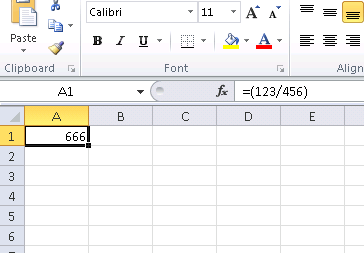
\includegraphics[width=0.6\textwidth]{digging_into_code/Excel_prank.png}
\caption{Der Scherz hat funktioniert}
\end{figure}

Wenn wir das gleiche mit der selben Excel Version versuchen, jedoch in 64-Bit Umgebungen.
Dann finden wir nur noch 12 \FDIV Instruktionen und die Instruktion nach der wir suchen ist
die dritte. 

\begin{lstlisting}
tracer.exe -l:excel.exe bpx=excel.exe!BASE+0x1B7FCC,set(st0,666)
\end{lstlisting}

\myindex{x86!\Instructions!DIVSD}

Es sieht danach aus als w\"aren viele der Division Operationen der \Tfloat und \Tdouble Typen, vom Compiler mit SSE Instruktionen ersetzt wurden.
Wie z.B \TT{DIVSD} (\TT{DIVSD} kommt insgesamt 268 mal vor).
